\section{Metode og gjennomføring}
\label{sec:metode}

Dette kapittelet beskriver hvordan studien er gjennomført, inkludert forskningsdesign, datainnsamling og analyse, prosjektgjennomføring og utviklingsmetodikk, samt hvordan den foreslåtte løsningen er evaluert. Prosjektets overordnede mål er å undersøke hvordan kunstig intelligens (AI) kan bidra til bedre søk og navigasjon på helsedirektoratet.no gjennom (i) kartlegging av dagens løsning, (ii) utvikling av et konsept/prototype, og (iii) evaluering av forbedringspotensialet. \cite{ProjectPlan}\footnote{Se også oppgaveteksten for bacheloroppgaven i vedlegg/innledning.}

Studien er strukturert i to komplementære forbedringsspor: (i) forbedret \textbf{søk} gjennom en backend-komponent med AI-støttet informasjonsgjenfinning og rangering, og (ii) forbedret \textbf{navigasjon} gjennom en frontend/GUI som reduserer friksjon i informasjonsflyten (bl.a.\ færre klikk og tydeligere veivalg). Begge sporene er forankret i funn fra kartleggingsfasen og evalueres samlet gjennom en sammenlikning mellom nåværende løsning og prototype.

\subsection{Forskningsdesign og metodisk tilnærming}
\label{sec:forskningsdesign}

Studien er gjennomført som en anvendt, designorientert undersøkelse hvor empirisk kartlegging kombineres med teknisk utvikling og evaluering. Tilnærmingen kan beskrives som en \textit{mixed methods}-studie: vi benytter både kvantitative og kvalitative datakilder for å forstå brukerbehov og utfordringer, og bruker dette som grunnlag for å designe og vurdere en forbedret løsning.

Metoden er tredelt:
\begin{enumerate}
    \item \textbf{Kartlegging av dagens løsning} gjennom primærdata (spørreundersøkelse) og sekundærdata (tidligere brukerinnsikt fra Helsedirektoratet).
    \item \textbf{Utvikling av prototype/konsept} som demonstrerer AI-assistert søk og navigasjon i en kontrollert, testorientert kontekst.
    \item \textbf{Evaluering av foreslått løsning} med fokus på relevans/treffsikkerhet, brukervennlighet og effektivitet, i tråd med oppgavens målsetning. \cite{ProjectPlan}
\end{enumerate}

I tråd med prosjektets rammer er løsningen utviklet som et \textit{proof of concept} og er ikke ment for produksjonssetting. Dette påvirker både valg av datakilder, modellstrategi og evalueringsdesign. \cite{ProjectPlan}

\subsection{Prosjektgjennomføring og utviklingsmetodikk}
\label{sec:gjennomforing}

Prosjektplanen, presentert i vedlegg \autoref{app:prosjektplan}, beskriver hvordan gjennomføringen opprinnelig var planlagt. Denne seksjonen oppsummerer hvordan arbeidet faktisk ble gjennomført i praksis. Selv om den overordnede metodikken ble fulgt, ble enkelte elementer justert underveis for å tilpasse arbeidsform, fremdrift og samarbeid med eksterne aktører.

\subsubsection{Utviklingsmodell}
\label{sec:scrum}

Prosjektet ble gjennomført med en smidig utviklingsmetodikk basert på Scrum, med GitHub Projects som scrumboard for sprintplanlegging og oppgaveoppfølging. Videre begrunnelse og mer detaljert prosess er beskrevet i prosjektplanen (vedlegg \autoref{app:prosjektplan}).

\begin{figure}[H]
    \centering
    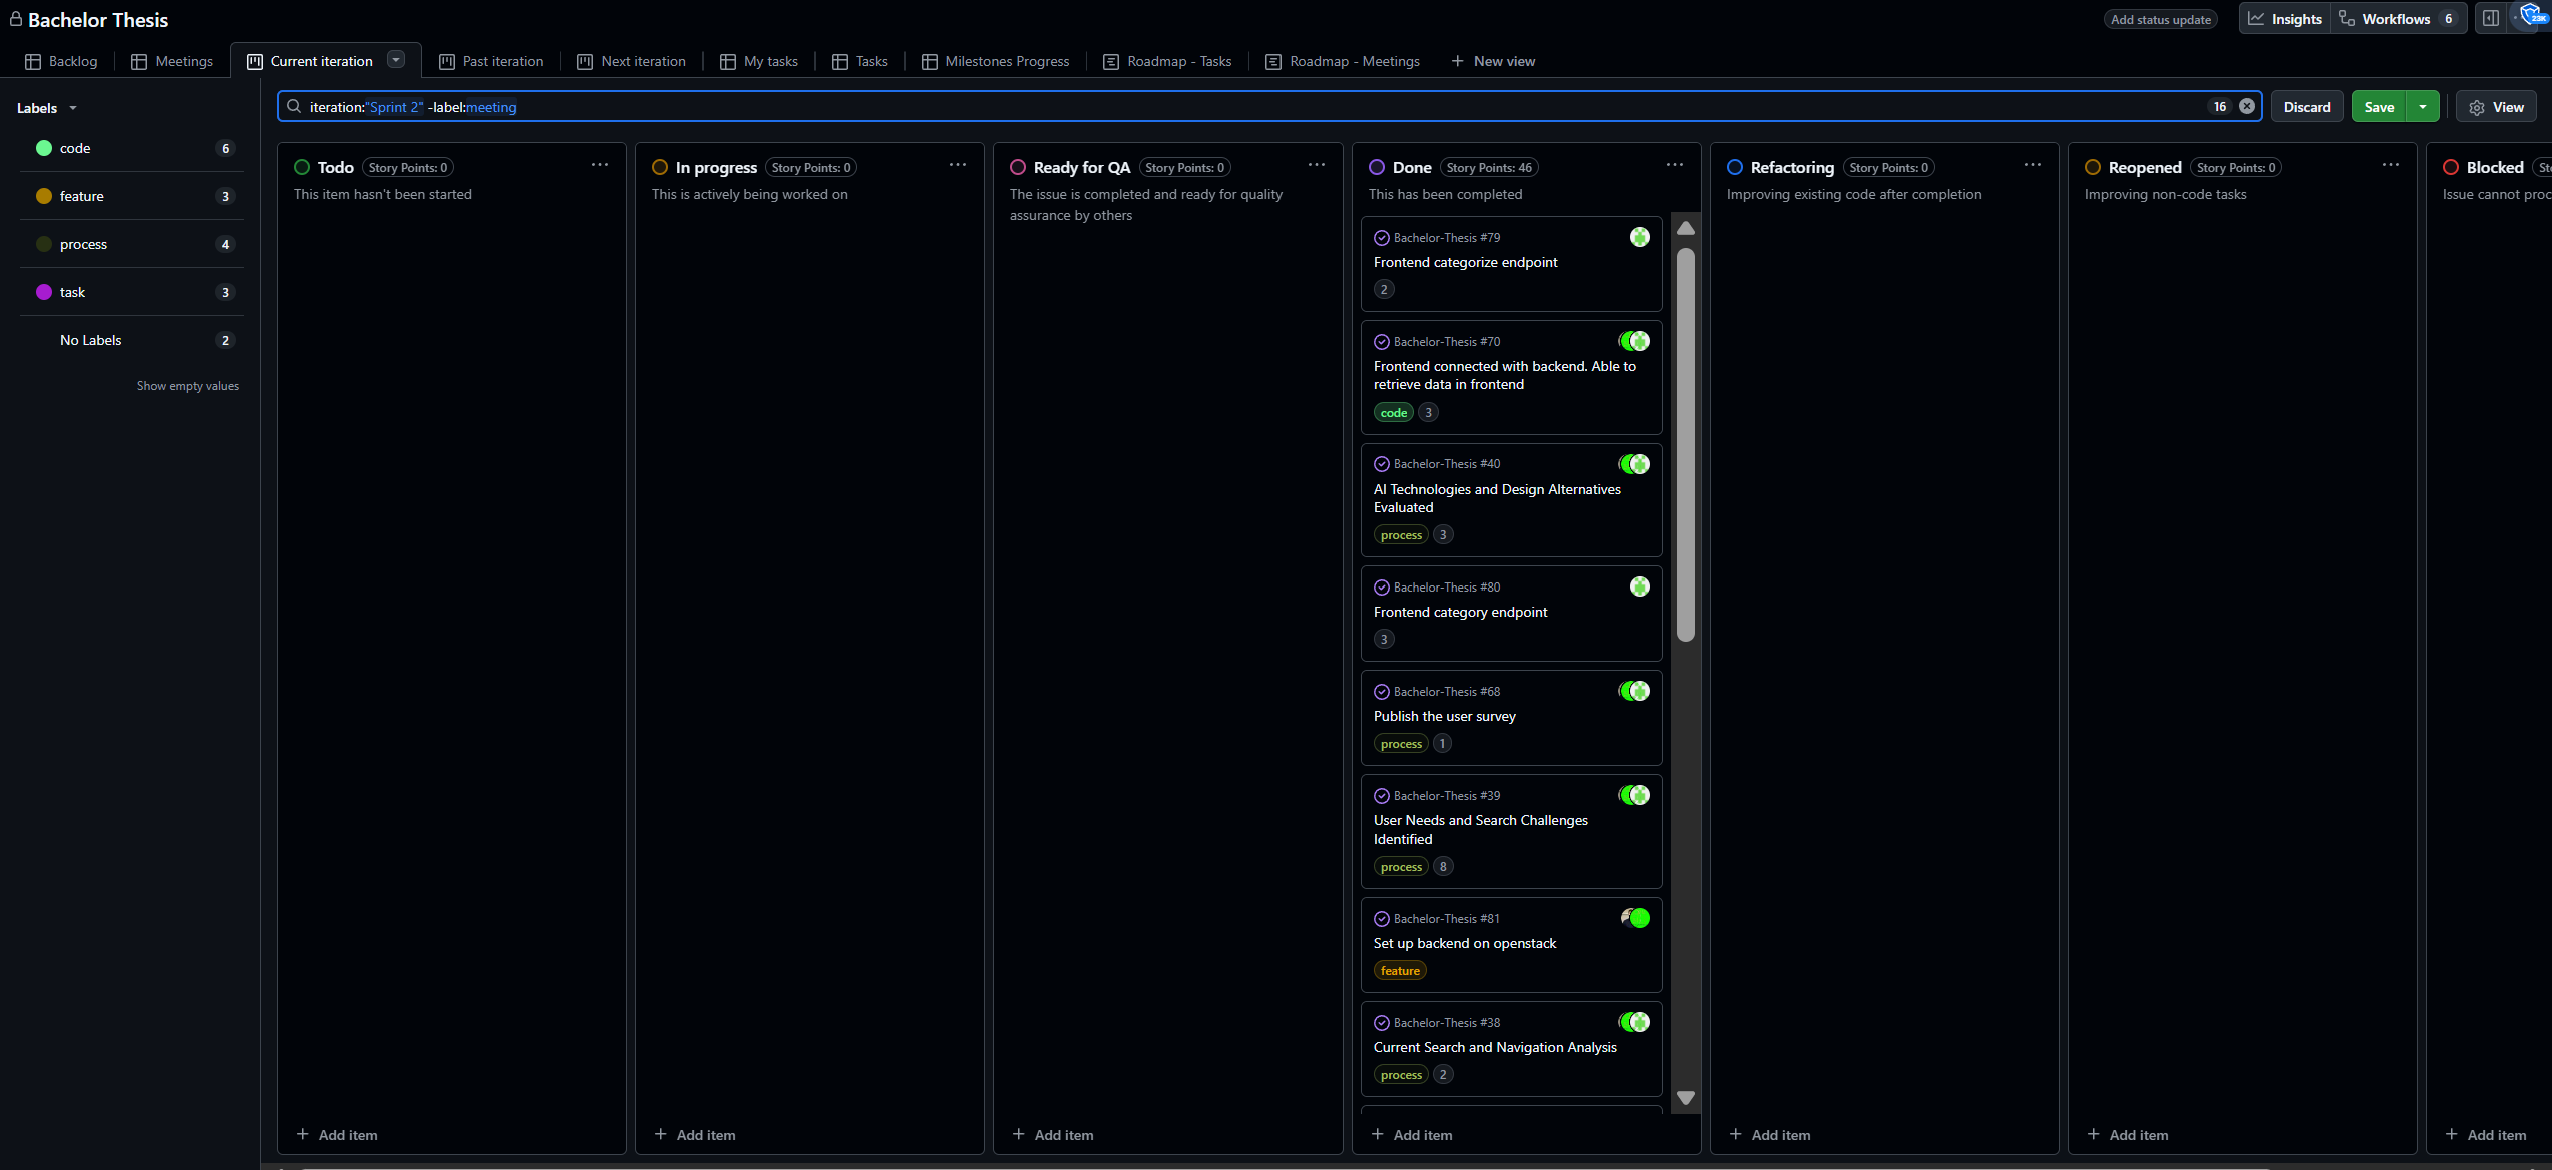
\includegraphics[width=\textwidth]{Images/ScrumBoard.png}
    \caption{Oversikt over GitHub Projects scrum board brukt til oppfølging av oppgaver og sprintplanlegging. Bildet viser eksempel på ferdigstilt sprint (Sprint 2).}
    \label{fig:github-projects-board}
\end{figure}

\subsubsection{Møtestruktur og koordinering}
\label{sec:moteflyt}

Daglige statusmøter (daily scrum) ble gjennomført kl.\ 09:15 fra mandag til fredag, primært fysisk når det var mulig. Møtene hadde kort varighet og fulgte en fast struktur hvor hvert medlem redegjorde for hva som var gjennomført siden forrige møte, hva som skulle arbeides med videre, og eventuelle hindringer. Denne rytmen bidro til kontinuerlig koordinering og tidlig identifisering av utfordringer i arbeidet.

Første dagen i hver sprint ble det gjennomført et sprintplanleggingsmøte (sprint planning) hvor oppgaver ble lagt inn i sprint backloggen. Deretter fikk oppgavene en estimert størrelse, prioritering og ble fordelt mellom gruppemedlemmene i tråd med sprintmålene. Ved slutten av hver sprint ble det gjennomført en sprintgjennomgang (sprint review) sammen med Product Owner. I disse møtene ble ferdigstilt funksjonalitet demonstrert og vurdert opp mot sprintmål, samtidig som teknologiske løsninger, metodiske valg og arkitektoniske vurderinger ble diskutert. Dette ga også grunnlag for å sammenholde prosjektets tilnærming med Helsedirektoratets rammebetingelser og pågående initiativer.

Etter sprintgjennomgangene ble det gjennomført interne sprintretrospektiver (sprint retrospective) i teamet. Her delte medlemmene hva de opplevde fungerte bra og mindre bra i sprinten. Formålet var å evaluere arbeidsflyt, samarbeidsprosesser og identifisere forbedringstiltak for neste sprint.

Hver onsdag ble det også holdt et møte med prosjektveilederen, der gruppens framdrift ble diskutert, og veileder ga tilbakemeldinger på arbeidet.

I tillegg til ordinære sprintmøter ble det i utvalgte sprinter arrangert utvidede demonstrasjoner med Helsedirektoratet, hvor flere interne representanter deltok. Disse møtene ga tverrfaglige tilbakemeldinger, økt innsikt i prosjektets fremgang og styrket interessentforankringen.

\subsubsection{Planverk og tidslinje}
\label{sec:gantt}

\begin{figure}[H]
    \centering
    \makebox[\textwidth][c]{%
        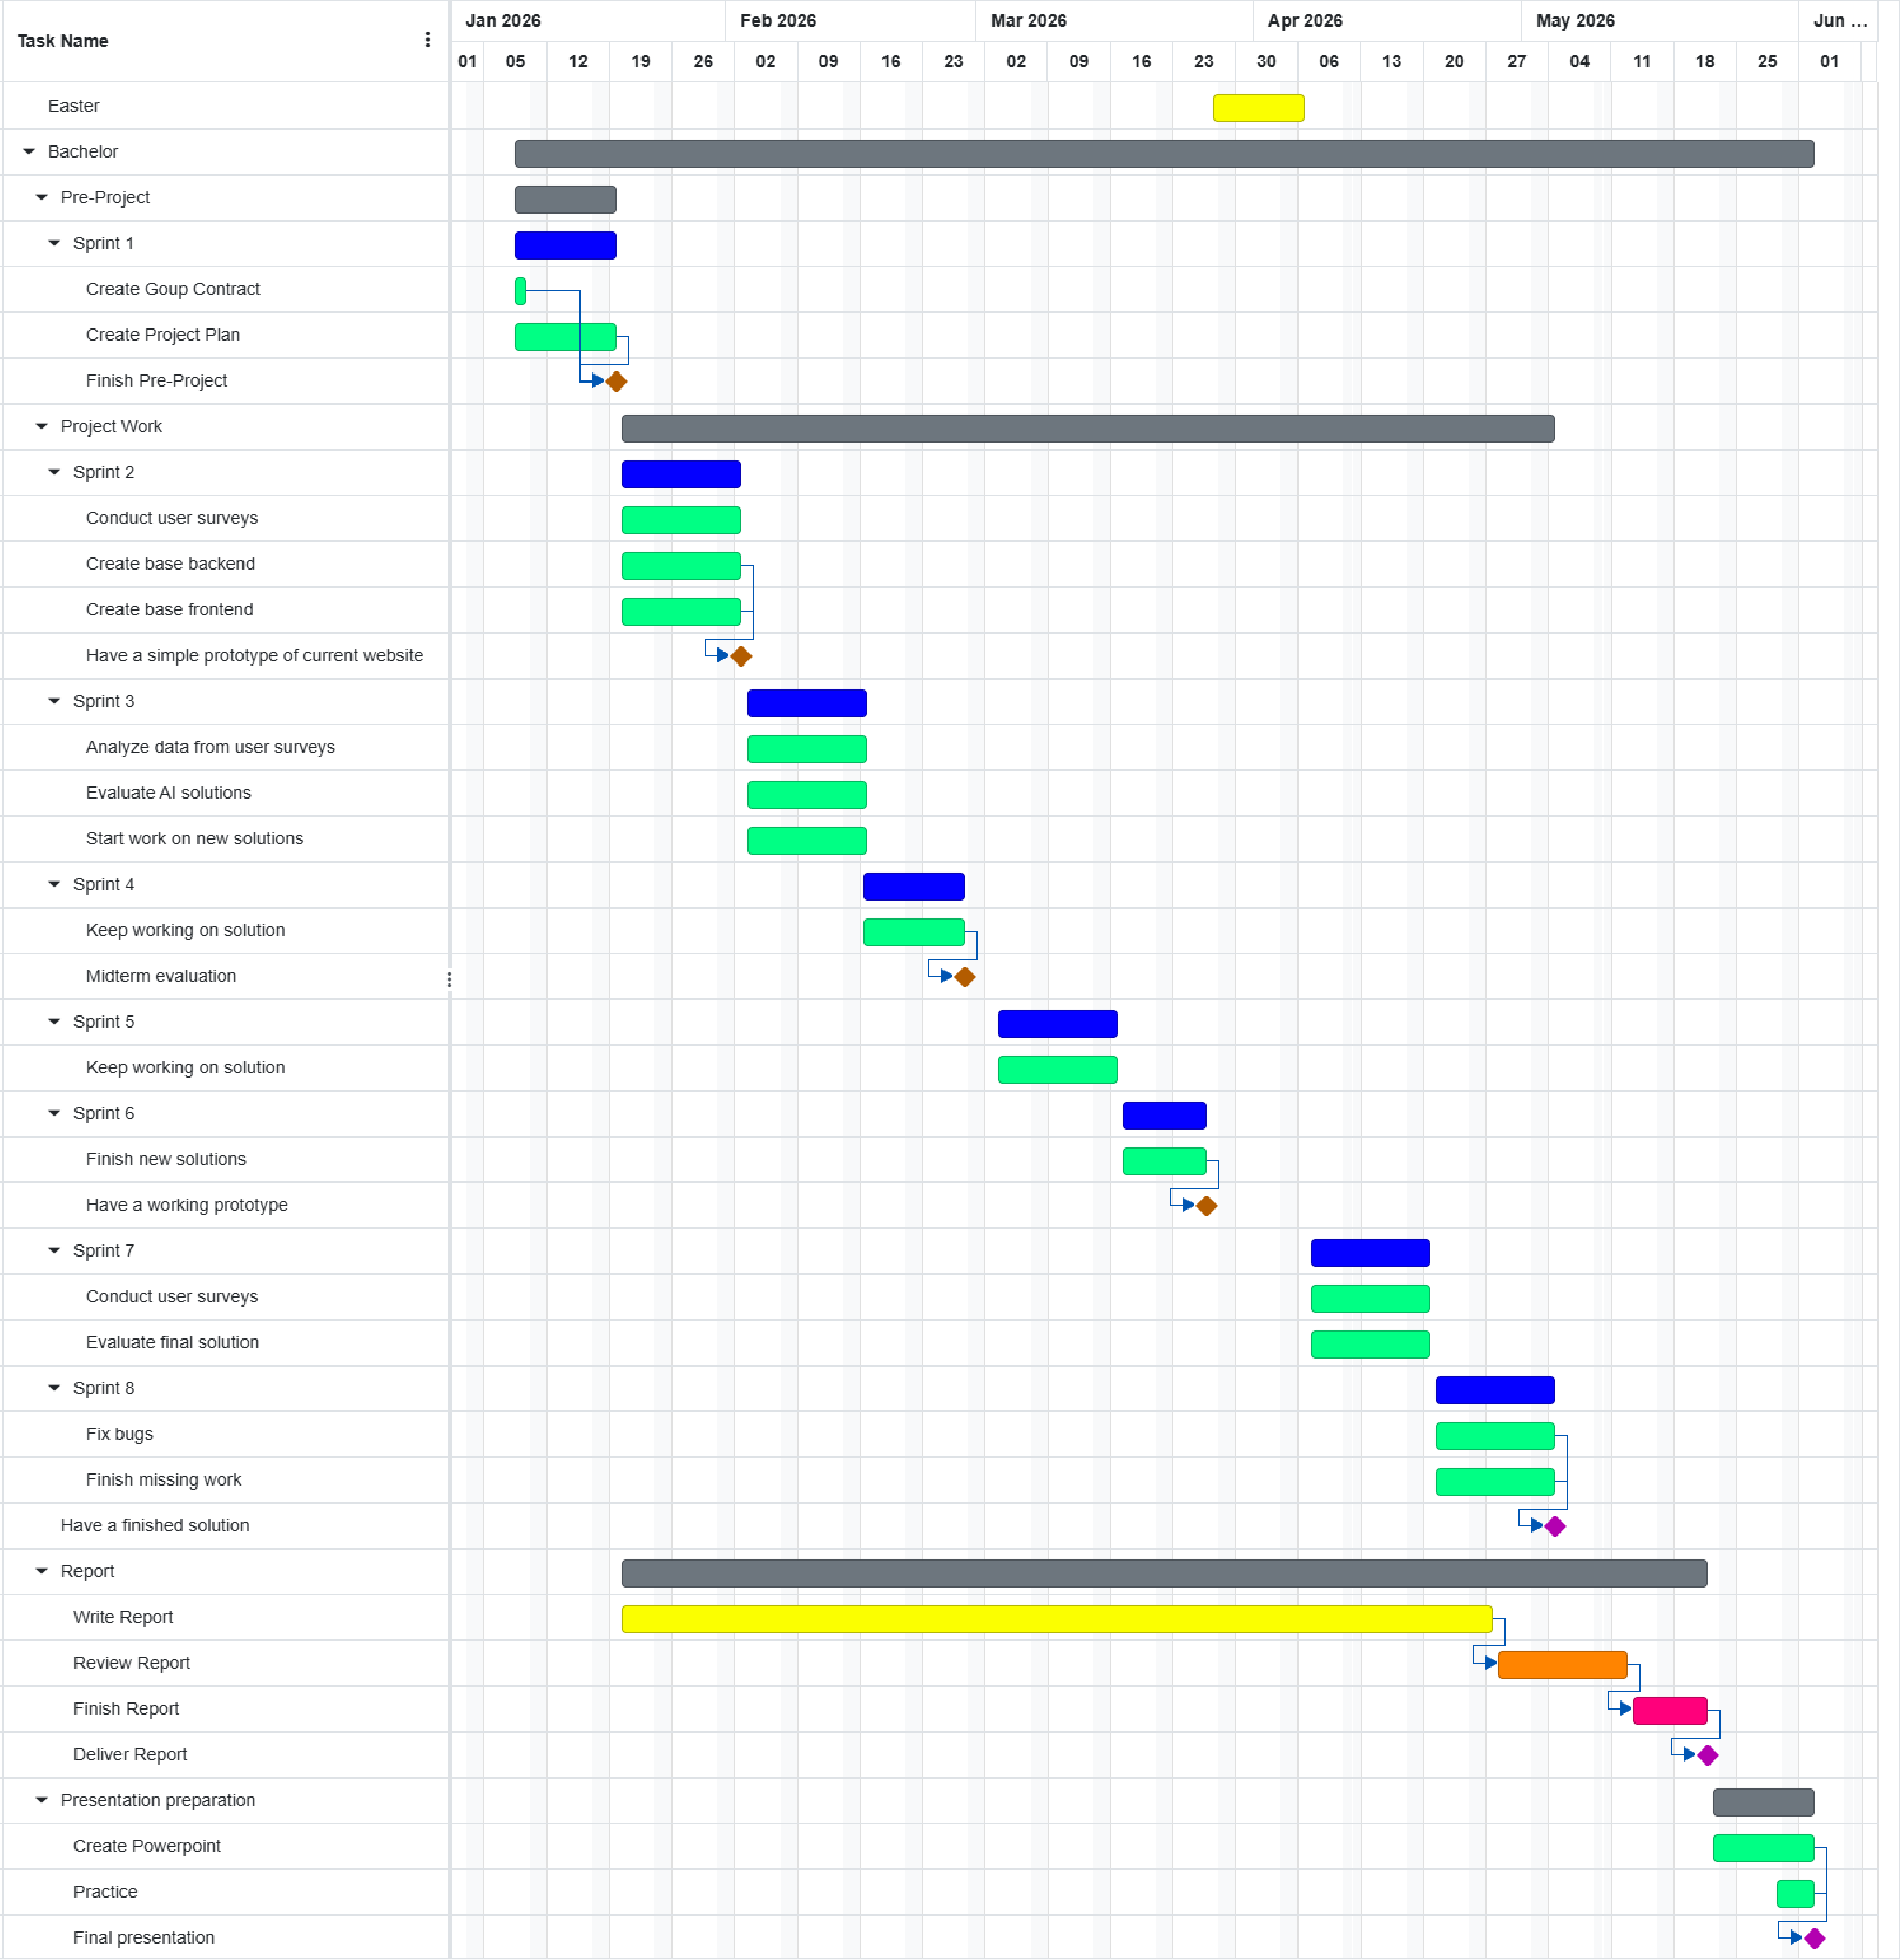
\includegraphics[width=1.2\textwidth]{Images/Gantt_diagram.pdf}
    }
    \caption{Gantt-diagram for prosjektet.}
    \label{fig:gantt-diagram}
\end{figure}

\subsubsection{Sammendrag av sprinter}
\label{sec:sprinter}

For å gi en overordnet fremdriftsbeskrivelse oppsummeres sentrale aktiviteter per sprint. Mer detaljert sprintlogg og oppgavehistorikk fremgår av GitHub Projects og prosjektplan (vedlegg \autoref{app:prosjektplan}).

\paragraph{Sprint 1 (5.\ jan -- 19.\ jan).}
Oppstartsfasen inkluderte laging av prosjektplan, etablering av samarbeidsrutiner (GitHub Projects, gruppekontrakt) og teknisk oppsett av utviklingsmiljø. Det ble gjennomført møter med Helsedirektoratet for å forstå kontekst og avklare oppgaveforståelse, og arbeidet med kartlegging (inkludert utforming av brukerundersøkelse) ble igangsatt.
%\subsection*{Sprint 1 (5. jan - 19. jan)}
%Starten av prosjektperioden gikk med på å lage prosjekt planen, sette opp github projects, lage gruppe kontrakt, sette opp backend, møte med helsedirektoratet og utforske deres oppsett og lage bruker undersøkelser. 

\paragraph{Sprint 2 (20.\ jan -- 2.\ feb).}
I sprint to arbeidet gruppen parallelt i frontend og backend. Det ble holdt flere møter med ansatte fra Helsedirektoratet for å avklare kravene til oppgaven, og det ble konkludert med at HAPI (Helsedirektoratets API) skulle brukes som kilde for innhold. Det ble satt opp en MySQL-database, og det ble hentet data fra HAPI til databasen. Videre ble API-endepunkter for søk og henting av innhold utviklet i backend, og frontend ble koblet mot disse for å vise søkeresultater og innhold. Det ble også opprettet en brukerundersøkelse i Microsoft Forms for evaluering av Helsedirektoratets nåværende løsning. Samtidig ble prosjektplanen finpusset slik at den var klar for levering innen fristen, og rapportens struktur ble utarbeidet. Mot slutten av sprinten nådde gruppen milepælen om å ha en enkel prototype av nettsiden.

\paragraph{Sprint 3 (3.\ feb -- 16.\ feb).}
I sprint tre ble det jobbet videre med både backend og frontend. På frontend ble søkesiden og sidene for innhold oppdatert, og det ble laget mulighet for å navigere frem til temasider fra hjemmesiden. Temasidene ble hentet inn fra Helsedirektoratet.no ved bruk av skript og lagt i databasen. For å forbedre søk ble det trent en embedding-modell på IDUN (NTNU sin superdatamaskin). Samtidig ble det satt opp digital infrastruktur på OpenStack med en VM for å hoste både frontend og backend, og disse ble koblet sammen ved bruk av GitHub Actions. Gruppen brukte også mye innsats på å samle svar på brukerundersøkelsen ved å sende e-poster til flere sykehus, møte opp på Sykehuset i Gjøvik, få den spredt internt hos Helsedirektoratet og få bekjente innen helsesektoren til å spre den. Parallelt ble arbeidet med rapporten påbegynt. Ved slutten av denne sprinten hadde gruppen mottatt 75 svar på brukerundersøkelsen.

\paragraph{Sprint 4 (17.\ feb -- 2.\ mar).}

\paragraph{Sprint 3--5 (3.\ feb -- 16.\ mar).}
Sprintene fokuserte videre på iterativ forbedring av datagrunnlag, søkekomponent og navigasjons-/presentasjonsløsning, samt forberedelse og gjennomføring av evaluering av prototypen. (Detaljer fylles inn når sprintene er ferdigstilt.)

\subsubsection{Logging av tidsbruk}
%Bruk av clockify + noen figurer

\subsection{Utvikling av programvare}

\subsubsection{Organisering av prosjekt i GitHub}
Hele prosjektet er organisert gjennom GitHub-organisasjonen ai-search-navigation-bachelor, som består av tre repositorier og ett GitHub-prosjekt. GitHub-prosjektet ble brukt til overordnet planlegging og organisering, inkludert kanban-tavle, møtelogg og sprintplanlegging. Repositoriet Bachelor-Report inneholdt en sikkerhetskopi av LaTeX-koden for rapporten, mens de to øvrige repositoriene, helsedir-ai-frontend og helsedir-ai-backend, var dedikert til henholdsvis frontend og backend.

Programkoden var dermed delt mellom to hovedrepositorier: ett for frontend og ett for backend. Frontend-repositoriet inneholdt koden til nettsiden som ble utviklet, og besto hovedsakelig av TypeScript- og React-kode. Backend-repositoriet inneholdt kode for serverlogikk, API-kall, modelltrening og tilhørende scripts, og var implementert i Python.

Begge repositoriene fulgte samme branch-struktur. En main-branch representerte produksjonsversjonen av systemet, og kode som ble merget til denne branchen ble automatisk deployert til en VM ved hjelp av GitHub Actions. I tillegg ble det brukt en dev-branch som integrasjons- og testgren, hvor nye funksjoner ble samlet før eventuell deployering. Nye feature-branches ble opprettet fra dev-branchen. Det var også satt opp automatiserte tester som ble kjørt ved opprettelse av Pull Requests (PR) til dev-branchen. Denne strukturen ble valgt for å sikre kontrollert integrasjon av nye funksjoner, god sporbarhet i utviklingsprosessen og stabil deploying av systemet.

\subsubsection{Arbeidsflyt for utvikling av kode}
Teamet fulgte en strukturert arbeidsflyt ved utvikling av ny funksjonalitet. Nye oppgaver ble først hentet fra sprint-backloggen i GitHub-prosjektet, der en valgt issue ble flyttet til In Progress og tildelt utvikleren dersom dette ikke allerede var gjort.

Deretter opprettet utvikleren en ny branch i riktig repositorium basert på den gjeldende versjonen av dev-branchen. Den planlagte funksjonaliteten ble så implementert i denne feature-branchen. Under utviklingsarbeidet ble det gjort løpende commits med korte, beskrivende meldinger. En del av koden ble utviklet med støtte fra KI-baserte kodeverktøy som Claude Code, ChatGPT eller GitHub Copilot.

Når funksjonaliteten var ferdig implementert, ble det opprettet en PR fra feature-branchen til dev-branchen. Ved opprettelse av PR ble det automatisk kjørt GitHub Actions som utførte enkle kvalitetskontroller. For frontend innebar dette blant annet lint-kontroll og type-sjekk. I tillegg mottok PR-en en automatisk kodegjennomgang fra CodeRabbit, som ga en oppsummering av endringer og forslag til mulige forbedringer eller feilrettinger.

Utvikleren gjennomgikk deretter resultatene fra testene og kodegjennomgangen, og gjorde nødvendige endringer før PR-en ble godkjent og merget til dev. Når dev-branchen inneholdt nye stabile funksjoner, ble det opprettet en ny Pull Request fra dev til main. Etter merging til main ble systemet automatisk deployert til den konfigurerte virtuelle maskinen via GitHub Actions. 


\subsection{Kartlegging: datagrunnlag og datainnsamling (baseline)}
\label{sec:kartlegging}

Formålet med kartleggingsfasen var å etablere et empirisk grunnlag for hvilke typer søk- og navigasjonsutfordringer brukere opplever på helsedirektoratet.no, og hvilke forbedringer som bør prioriteres i en KI-assistert løsning.

\subsubsection{Primærdata: spørreundersøkelse}
\label{sec:survey}

Primærdata ble samlet inn gjennom en kvantitativ spørreundersøkelse utformet i Microsoft Forms\footnote{\url{https://forms.office.com}}. Skjemaet er vedlagt i \autoref{app:forms} og inneholder både lukkede og åpne spørsmål for å kombinere målbare vurderinger med fritekstbasert brukerinnsikt.

Spørsmålene dekker blant annet respondentens rolle, bruksfrekvens og formål med besøk, vurdering av søk og navigasjon på skala, opplevde utfordringer, samt forslag til forbedringer. Undersøkelsen var anonym, og det ble ikke samlet inn personidentifiserende opplysninger.

Utformingen av spørreundersøkelsen ble kvalitetssikret gjennom samarbeid med interaksjonsdesigner Christine Hørven i Helsedirektoratet, som arbeider med brukerundersøkelser knyttet til helsedirektoratet.no. Hun ga konkrete tilbakemeldinger på spørsmålsformuleringer, struktur og relevans før distribusjon. Dette bidro til å styrke undersøkelsens faglige forankring og sikre at spørsmålene var tilpasset kjente brukerbehov på nettstedet.

\subsubsection{Rekruttering og utvalg}
\label{sec:utvalg}

Målsettingen var å nå et bredt spekter av brukere som representerer sentrale målgrupper for helsedirektoratet.no, slik som helsepersonell, kommunal/offentlig sektor og privatpersoner. Opprinnelig var planlagt distribusjon via \textit{Skyra.no}\footnote{\url{https://www.skyra.no/no}} gjennom Helsedirektoratets flater, slik at undersøkelsen kunne vises til tilfeldig utvalgte besøkende på nettstedet. Denne løsningen lot seg imidlertid ikke gjennomføre innenfor prosjektperioden, blant annet fordi det allerede pågikk andre brukerundersøkelser på nettstedet.

Som alternativ ble undersøkelsen distribuert gjennom flere supplerende kanaler. Christine Hørven bidro til deling av undersøkelsen i relevante interne kommunikasjonskanaler i Helsedirektoratet. I tillegg ble undersøkelsen sendt direkte via e-post til flere helseinstitusjoner og sykehus i Norge. Til tross for at mange sykehus ble kontaktet, resulterte dette i svært få svar, og flere ga tilbakemelding om at de ikke hadde anledning til å distribuere undersøkelsen internt.

Gruppen benyttet også faglige og personlige nettverk for å nå potensielt relevante respondenter, og oppfordret mottakere til videre deling av undersøkelsen (snowball-rekruttering). Det ble også gjennomført et fysisk besøk ved Sykehuset i Gjøvik for å informere om undersøkelsen, selv om dette i begrenset grad resulterte i flere svar.

Rekrutteringsstrategien innebærer et \textit{ikke-sannsynlighetsutvalg} (convenience/snowball), noe som gir kontekstnær innsikt i brukernes erfaringer, men begrenser generaliserbarheten av funnene (se \autoref{sec:validitet}).

\subsubsection{Sekundærdata}
\label{sec:sekundaerdata}

Prosjektgruppen har i tillegg hatt tilgang til eksisterende brukerinnsikt og tidligere undersøkelser fra Helsedirektoratet. Disse fungerer som sekundærdata og brukes som sammenligningsgrunnlag for å vurdere om identifiserte utfordringer fremstår som vedvarende, samt for å triangulere funn fra vår egen kartlegging.

\subsubsection{Databehandling og analysemetoder}
\label{sec:analyse} 

Analysen ble gjennomført i to spor, tilpasset datatypene i undersøkelsen.

\subsubsection*{Kvantitativ analyse}
\label{sec:kvant}

Lukkede spørsmål (skala- og flervalgsspørsmål) ble analysert deskriptivt ved hjelp av frekvenser, fordelinger og sentralmål (f.eks.\ gjennomsnitt/median der det var hensiktsmessig). Formålet var å identifisere mønstre i opplevd kvalitet på søk og navigasjon, og avdekke hvilke utfordringer som forekommer hyppigst.

\subsubsection*{Kvalitativ analyse}
\label{sec:kval}

Åpne svar ble analysert tematisk ved å kode gjentakende mønstre i opplevde utfordringer, behov og forbedringsforslag. Kodene ble deretter gruppert til overordnede tema som brukes som designgrunnlag for prototypen og som støtte i diskusjonen.

\subsection{Evalueringsopplegg (baseline--prototype)}
\label{sec:evaluering}

Evalueringen er gjennomført for å vurdere om prototypen kan gi målbar eller opplevd forbedring i søk og navigasjon, i tråd med prosjektets effektmål (relevans, tidsbruk, opplevd brukervennlighet og mer konsistent organisering). \cite{ProjectPlan}

\subsubsection{Evalueringskriterier}
\label{sec:kriterier}

Evalueringen tar utgangspunkt i kriterier knyttet til treffsikkerhet og relevans, brukervennlighet og navigasjonsstøtte, transparens og effektivitet. Disse operasjonaliseres i kapittel \ref{sec:resultater} gjennom mål på oppgavegjennomføring og brukeropplevelse.

\subsubsection{Evalueringsprotokoll}
\label{sec:opplegg}

Evalueringen er lagt opp som en baseline--prototype-sammenlikning: nåværende løsning (helsedirektoratet.no) brukes som referansepunkt, og prototypen vurderes opp mot representative informasjonsbehov og søkeoppgaver. Der det har vært mulig er sammenligningen støttet av både skala-/vurderingsspørsmål og kvalitative tilbakemeldinger.

\subsection{Validitet, pålitelighet og begrensninger}
\label{sec:validitet}

Studien har flere forhold som påvirker tolkning og generaliserbarhet. Rekruttering gjennom tilgjengelige kanaler gir verdifull innsikt, men innebærer selvseleksjon og mulig skjevhet i hvilke brukergrupper som deltar. Spørreundersøkelsen gir bredde, men fanger primært selvrapportert adferd. Videre er løsningen et proof-of-concept og kan avvike fra forventninger brukere har til helsedirektoratet.no i produksjonsmiljø. Resultater fra evalueringen må derfor forstås som en vurdering av potensial og retning, ikke endelig effekt i drift. \cite{ProjectPlan}

\subsection{Etiske hensyn}
\label{sec:etikk}

Etiske hensyn er særlig relevante gitt at løsningen omhandler helseinformasjon og offentlig forvaltning. Studien har ivaretatt personvern ved anonym datainnsamling, og prosjektet legger til grunn et prinsipp om at AI-støtte skal være forankret i verifiserbare kilder for å redusere risiko for feil eller misledende informasjon. Videre vektlegges transparens i presentasjon av resultater, slik at brukeren kan forstå og etterprøve treffene, og slik at potensielle skjevheter kan identifiseres og diskuteres.
%Vi har anonyme brukerundersøkelser

